\section{Introdução}\label{sec:introducao}
Decisões arquiteturais organizam responsabilidades e dependências e afetam
como equipes desenvolvem e verificam um sistema. Entretanto, reconhecer um
padrão no código não demonstra, por si só, melhoria de qualidade. É necessário
relacionar a decisão a interesses, perguntas e evidências.

Este trabalho analisa o Now in Android (NiA), projeto aberto do Google que
serve de referência para desenvolvimento Android~\cite{nowinandroid,android-arquitetura}. O
objetivo é identificar suas decisões arquiteturais e aplicá-las, com
simplificações justificadas, a uma demonstração de notícias e favoritos.
O método consiste em inspeção estática de uma revisão fixada, análise dos
stakeholders, construção de vistas e de um plano Goal/Question/Metric
(GQM), seguida de implementação e testes de um aplicativo independente.
As medições executadas pertencem exclusivamente à demonstração.

A Seção~\ref{sec:fundamentacao} apresenta os conceitos utilizados e a
Seção~\ref{sec:metodos}, o método. As Seções~\ref{sec:projeto} a
\ref{sec:diagramas} caracterizam o NiA e analisam stakeholders, vistas,
qualidade e arquitetura. A Seção~\ref{sec:projeto-base} descreve a
demonstração e seus resultados, discutidos na Seção~\ref{sec:discussao}; a
Seção~\ref{sec:conclusao} conclui o trabalho.

\begin{figure*}[t]
\centering
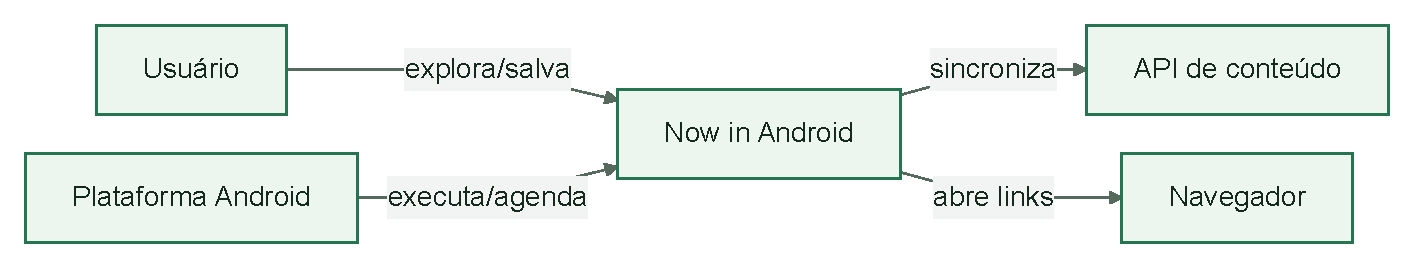
\includegraphics[width=\textwidth]{imagens/01-contexto.pdf}
\caption{Contexto do NiA: interação do leitor, conteúdo remoto, navegação
externa e serviços da plataforma. Armazenamentos internos são detalhados nas
outras vistas.}
\Description{O usuário explora o aplicativo; o aplicativo sincroniza com a API e abre links no navegador; a plataforma Android executa e agenda trabalho.}
\label{fig:contexto}
\end{figure*}
